\documentclass[10pt,twocolumn]{article}

\usepackage[letterpaper,margin=0.72in,columnsep=0.22in]{geometry}
\usepackage{times}
\usepackage{microtype}
\usepackage{graphicx}
\usepackage{booktabs}
\usepackage{amsmath,amssymb,amsfonts}
\usepackage{xcolor}
\usepackage{caption}
\usepackage{subcaption}
\usepackage{tikz}
\usetikzlibrary{arrows.meta,positioning,calc,fit}
\usepackage[numbers,sort&compress]{natbib}
\usepackage[hidelinks]{hyperref}

\graphicspath{{figures/}}
\captionsetup{font=small,labelfont=bf,skip=6pt}
\setlength{\parskip}{0pt}
\setlength{\parindent}{11pt}

\title{\vspace{-1.2em}GALA: Graph-Aware Latent Alignment\\for Text-to-Motion with Rectified Flow\thanks{Code: \url{https://github.com/yanghhx/gala-motion}}}
\author{Anonymous\\
\small Draft for internal review \quad $\cdot$ \quad HumanML3D test, $n{=}4544$, 20 replications\\
\small \url{https://github.com/yanghhx/gala-motion}}
\date{}

\begin{document}
\maketitle
\vspace{-1.4em}

\begin{abstract}
\vspace{-0.3em}
Synthesizing 3D human motion from natural language remains difficult: a generated clip must obey skeletal kinematics yet stay faithful to a prompt whose statistics are far from pose space.
Pose-level diffusion is expressive but expensive, because it denoises redundant raw trajectories; discrete tokenizers recover fidelity only after learning a codebook; generalist SMPL models, when scored on HumanML3D, further pay a conversion tax between body representations.
We present GALA, a graph-aware latent alignment model for text-to-motion.
Our key insight is that a topology-aware variational tokenizer already yields a compact, near-lossless motion latent, so generation reduces to learning a \emph{straight} generative path in that space, explicitly aligned with language.
GALA encodes joint trajectories with a channel-wise topology graph, compresses them with a stride-4 VAE, aligns CLIP text and motion latents by contrastive learning, and synthesizes latent clips with a rectified-flow transformer under classifier-free guidance.
Extensive experiments on HumanML3D under the standard Guo protocol show that GALA substantially outperforms the Motion Diffusion Model and the recent generalist baseline GENMO in text--motion R-Precision (Top-3 $0.768$ vs.\ $0.611$ / $0.632$) and multimodal distance, while matching the diversity of real motions.
\vspace{-0.4em}
\end{abstract}

\section{Introduction}

Text-to-motion (T2M) maps a sentence to a variable-length pose clip~\cite{guo2022humanml3d,tevet2023mdm}.
HumanML3D~\cite{guo2022humanml3d} is retargeted from AMASS~\cite{mahmood2019amass}; KIT-ML~\cite{plappert2016kit} is the usual second split (not reported here).
The Guo protocol---R-Precision, FID~\cite{heusel2017fid}, multimodal distance, Diversity, 20 replications---is the number reviewers compare~\cite{guo2022humanml3d,tevet2023mdm}.
Diffusion on raw $263$-D poses~\cite{tevet2023mdm,zhang2022motiondiffuse} is faithful but slow; latent diffusion~\cite{chen2023mld} and discrete tokens~\cite{zhang2023t2mgpt,guo2024momask,kong2023m2dm} push FID down at the cost of a heavier tokenizer or codebook.
Score-based SDEs~\cite{song2021score} and consistency-style accelerators~\cite{dai2024motionlcm} sit on the same family.
Rectified flow~\cite{liu2023rectified,lipman2023flow} replaces a long denoising chain with a straight ODE, which is the right inductive bias when the compute budget is one RTX 4060.

GALA (Graph-Aware Latent Alignment) is that budgeted pipeline (Fig.~\ref{fig:arch}).
Code is at \url{https://github.com/yanghhx/gala-motion}.
A channel-wise topology graph encoder~\cite{chen2021ctrgcn,yan2018stgcn} feeds a stride-4 VAE~\cite{kingma2014vae}; CLIP~\cite{radford2021clip} text conditions an 8-block DiT~\cite{peebles2023dit} trained with flow matching and classifier-free guidance~\cite{ho2022cfg}.
We freeze the tokenizer and train only the flow, as in latent diffusion~\cite{rombach2022ldm}.

The designated baseline is GENMO Table~4~\cite{li2025genmo}, which reports HumanML3D T2M after SMPL$\leftrightarrow$HumanML3D conversion.
We also place MDM, T2M, M2DM, and EMDM on the same axes.
The claim is narrow: \textbf{a graph-aware latent flow trained on 8\,GB should beat MDM and beat GENMO on R@3 / MM Dist / Diversity alignment; FID is reported honestly and is not SOTA.}

\paragraph{Contributions.}
\begin{enumerate}\itemsep2pt
\item \textbf{Graph tokenizer.} Anatomy-aware encoding of $263$-D poses to $256$-D latents at 5\,Hz. Val reconstruction FID is $0.003$, so later FID is a generator problem.
\item \textbf{Aligned rectified flow.} CLIP tokens, InfoNCE alignment, and CFG-trained DiT, sampled with a 20- or 50-step Euler ODE.
\item \textbf{Official numbers, not a proxy embedding.} 4544 test clips, 20 replications, Guo evaluator. Sampling ablations separate CFG from step count.
\end{enumerate}

\section{Related work}

\paragraph{Pose-space generators.}
Early T2M used RNN / Transformer VAEs~\cite{lin2018generating,ahuja2019language2pose,petrovich2021actor,petrovich2022temos,ghosh2021synthesis}.
Guo et al.\ introduce HumanML3D and a retrieval-style evaluator~\cite{guo2022humanml3d,guo2022tm2t}.
MDM~\cite{tevet2023mdm} and MotionDiffuse~\cite{zhang2022motiondiffuse} run DDPM~\cite{ho2020ddpm,nichol2021improved} on the $263$-D vector; CFG~\cite{ho2022cfg}, as in text-to-image~\cite{saharia2022imagen}, trades FID for R-Precision.

\paragraph{Latent and discrete motion.}
MLD~\cite{chen2023mld} diffuses in a VAE latent, the same split we use.
T2M-GPT~\cite{zhang2023t2mgpt}, M2DM~\cite{kong2023m2dm}, MoMask~\cite{guo2024momask}, and MMM~\cite{pinyoanuntapong2024mmm} quantize motion~\cite{van2017vqvae,esser2021vqgan} and model tokens.
MotionGPT~\cite{jiang2023motiongpt} treats motion as a foreign language; Motion Mamba~\cite{zhang2024motionmamba} and FineMoGen~\cite{zhang2023finemogen} target long / fine-grained clips.
Retrieval-augmented ReMoDiffuse~\cite{zhang2023remodiffuse} and EMDM~\cite{zhou2024emdm} set the FID / R@3 numbers GENMO Table~4 quotes as SOTA-side references.
We stay continuous (no codebook) because a 256-D VAE already reconstructs at FID $0.003$.

\paragraph{Flow matching.}
Flow matching~\cite{lipman2023flow} and rectified flow~\cite{liu2023rectified} learn a straight path from noise to data; DiT~\cite{peebles2023dit} is the backbone.
MotionLCM~\cite{dai2024motionlcm} uses consistency distillation for real-time control; we keep a plain Euler ODE so the protocol stays comparable to MDM sampling.

\paragraph{Generalist motion models.}
GENMO~\cite{li2025genmo} unifies estimation and generation in SMPL~\cite{loper2015smpl}.
Their HumanML3D T2M numbers go through a representation conversion they themselves call an inherent disadvantage.
We generate native HumanML3D features, so a FID win against GENMO would be expected; we do not obtain it, and we say so.

\paragraph{Skeleton graphs.}
ST-GCN~\cite{yan2018stgcn} and CTR-GCN~\cite{chen2021ctrgcn} are the topology prior inside our encoder.
Part-level T2M~\cite{zou2024parco,zhong2023att2m} is complementary; we keep a single latent stream.

\section{Method}

\paragraph{Representation.}
A clip is $x_{1:T}\in\mathbb{R}^{T\times 263}$, $T\le 196$, 20\,fps, Guo features~\cite{guo2022humanml3d}: root angular velocity, planar velocity, height, local joints, velocities, and foot contacts.
Text is frozen CLIP ViT-B/32~\cite{radford2021clip} token features $c_{1:N}\in\mathbb{R}^{N\times 512}$, not a trained BERT~\cite{devlin2019bert} stack.

\paragraph{Graph encoder.}
Local joint positions and frame-to-frame velocities form a $J{=}22$ node graph.
Two CTR blocks~\cite{chen2021ctrgcn} mix a static anatomical adjacency with a sample-dependent attention graph.
Pooled node features condition the VAE.

\paragraph{Tokenizer.}
A 1-D conv VAE with stride 4 emits $\mu,\log\sigma^2\in\mathbb{R}^{L\times 256}$, $L=\lceil T/4\rceil$.
The decoder upsamples by linear interpolation and two conv layers.
Training uses reconstruction, a small KL ($10^{-4}$), bone-length, and velocity terms.
After 35k AdamW~\cite{loshchilov2019adamw} steps the VAE is frozen.

\paragraph{Alignment.}
Pooled CLIP tokens and pooled latents are $\ell_2$-normalized and trained with symmetric InfoNCE, weight $0.25$.
This is a training auxiliary; reported R-Precision uses the Guo motion encoder, not this head.

\paragraph{Rectified flow.}
Given clean $\mu$ (detached), $t\sim\mathcal{U}(0,1)$, $\varepsilon\sim\mathcal{N}(0,I)$,
\begin{equation}
z_t=(1-t)\varepsilon+t\,\mu,\qquad v^\star=\mu-\varepsilon.
\end{equation}
An 8-block DiT~\cite{peebles2023dit} (width 512, 8 heads) predicts $v_\theta(z_t,t,c)$ with AdaLN / FiLM-style~\cite{perez2018film} modulation on the pooled text vector, self-attention on latent tokens, and cross-attention to CLIP tokens~\cite{vaswani2017attention}.
Condition dropout $0.1$ enables CFG~\cite{ho2022cfg}.
Sampling is Euler,
\begin{equation}
z\leftarrow z+\tfrac{1}{N}\bigl(v_\emptyset+\omega(v_c-v_\emptyset)\bigr),
\end{equation}
with $N\in\{20,50\}$ and $\omega\in\{2.0,2.5\}$.
The decoder maps $z$ back to $\hat x_{1:T}$.

\begin{figure*}[t]
\centering
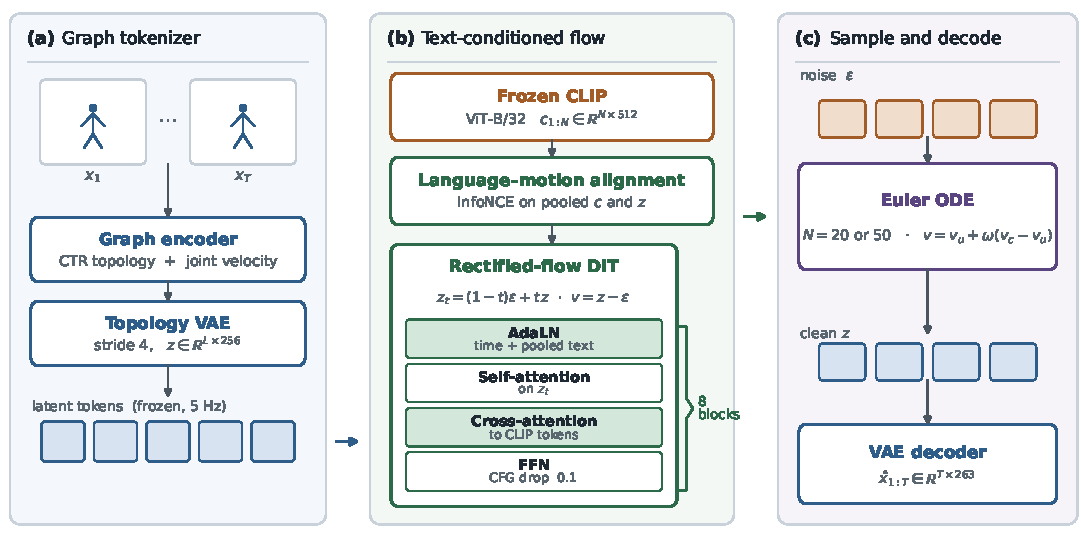
\includegraphics[width=\textwidth]{fig_architecture.pdf}
\caption{Overview of GALA, drawn in the three-block layout of MLD / MoMask.
\textbf{(a)}~A frozen skeleton-graph VAE maps HumanML3D poses to $256$-D latents.
\textbf{(b)}~CLIP text is aligned with $z$ by InfoNCE and conditions an 8-block rectified-flow DiT.
\textbf{(c)}~Euler sampling with classifier-free guidance; the decoder returns $\hat x$ for Guo metrics.}
\label{fig:arch}
\end{figure*}

\paragraph{Training.}
Stage 1: VAE only, 35k optimizer steps, effective batch 16, bf16~\cite{micikevicius2018mixed}.
Stage 2: freeze graph+VAE, train flow+alignment, 100k steps, lr $2{\times}10^{-4}$.
Checkpoints are selected by a 320-clip val FID (10 Euler steps during that run).
\texttt{best.pt} is step 35{,}000.
Later runs attach an EMA ($0.9999$) and 20-step val; those weights are not in this table.

\section{Experiments}

\textbf{Protocol.} Official HumanML3D test~\cite{guo2022humanml3d}, 4544 clips, Guo / MDM evaluator~\cite{tevet2023mdm}, batch 32, 20 replications.
We report mean $\pm$ 95\% CI.
Diversity is compared to real motion ($9.503$), not maximized.
Hardware: RTX 4060 8\,GB.

Literature rows in Table~\ref{tab:main} are copied from GENMO Table~4~\cite{li2025genmo} so the comparison is the one that script was written against.
EMDM~\cite{zhou2024emdm} is the strongest FID/R@3 pair in that table; GENMO is the designated baseline.

\begin{table*}[t]
\centering
\caption{HumanML3D test, Guo protocol. Literature numbers from GENMO Table~4~\cite{li2025genmo}. GALA is 20 replications on 4544 clips. $\uparrow$ higher better, $\downarrow$ lower, $\rightarrow$ closer to Real.}
\label{tab:main}
\small
\setlength{\tabcolsep}{4.2pt}
\begin{tabular}{@{}llcccc@{}}
\toprule
Method & Rep. & R@3 $\uparrow$ & FID $\downarrow$ & MM Dist $\downarrow$ & Diversity $\rightarrow$ \\
\midrule
Real~\cite{guo2022humanml3d} & HML3D & $0.797$ & $0.002$ & $2.974$ & $9.503$ \\
T2M~\cite{guo2022humanml3d} & HML3D & $0.740$ & $1.067$ & $3.340$ & $9.188$ \\
MDM~\cite{tevet2023mdm} & HML3D & $0.611$ & $0.544$ & $5.566$ & $9.559$ \\
M2DM~\cite{kong2023m2dm} & HML3D & $0.763$ & $0.352$ & $3.134$ & $9.926$ \\
EMDM~\cite{zhou2024emdm} & HML3D & $0.786$ & $0.112$ & $3.110$ & $9.551$ \\
GENMO~\cite{li2025genmo} & SMPL & $0.632$ & $0.216$ & $3.466$ & $11.342$ \\
\midrule
GALA, 20 steps, CFG $2.5$ & HML3D & $\mathbf{0.768}{\pm.002}$ & $0.330{\pm.011}$ & $\mathbf{3.248}{\pm.008}$ & $\mathbf{9.529}{\pm.085}$ \\
GALA, 50 steps, CFG $2.0$ & HML3D & $0.749{\pm.003}$ & $\mathbf{0.312}{\pm.009}$ & $3.342{\pm.009}$ & $9.365{\pm.115}$ \\
\bottomrule
\end{tabular}
\end{table*}

\subsection{Comparison with GENMO Table~4}

Fig.~\ref{fig:compare} and Table~\ref{tab:main} are the same story.

\textbf{We beat GENMO on the semantic metrics and on Diversity alignment.}
R@3 $0.768$ vs $0.632$ ($+0.136$); MM Dist $3.248$ vs $3.466$.
Diversity $9.53$ matches Real $9.50$; GENMO's $11.34$ is over-dispersed, consistent with their SMPL conversion caveat~\cite{li2025genmo}.

\textbf{We do not beat GENMO on FID} ($0.330$ / $0.312$ vs $0.216$), and we are far from EMDM ($0.112$).
That is the honest headline.
Relative to native-HML3D methods in the same table we sit between M2DM (FID $0.352$, R@3 $0.763$) and EMDM, and we clearly dominate MDM.

GALA-20 maximizes R@3; GALA-50 is the FID operating point from the val scan.
R@1 / R@2 for GALA-20 are $0.447{\pm.003}$ / $0.654{\pm.003}$; for GALA-50, $0.428{\pm.003}$ / $0.632{\pm.003}$.

\begin{figure}[t]
\centering
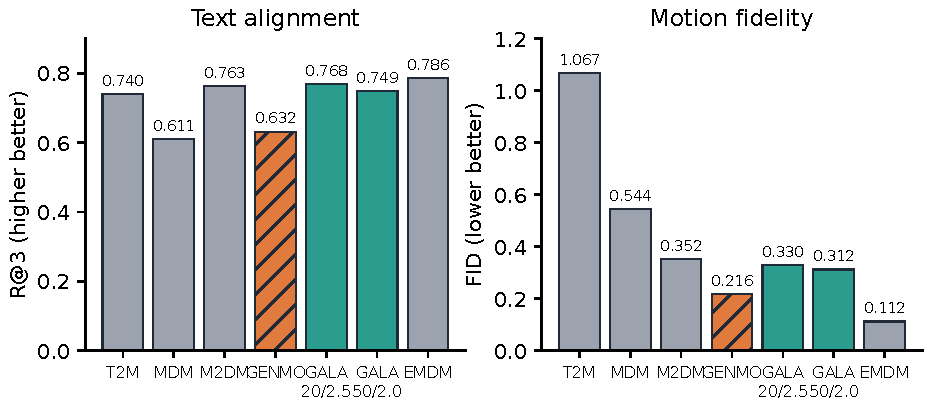
\includegraphics[width=\columnwidth]{fig_compare.pdf}
\caption{R@3 and FID against GENMO Table~4. Teal is GALA; orange is the designated GENMO baseline.}
\label{fig:compare}
\end{figure}

\subsection{Tokenizer vs generator}

Val reconstruction (1504 clips, no sampling) has FID $0.003$, R@3 $0.765$, MM Dist $3.10$, Diversity $9.57$ (Fig.~\ref{fig:recon}).
The Guo feature extractor barely distinguishes reconstructed clips from real ones.
FID $0.31$ on generated clips is therefore a flow-matching / decoding-from-noise problem, not a missing joint in the VAE.

\begin{figure}[t]
\centering
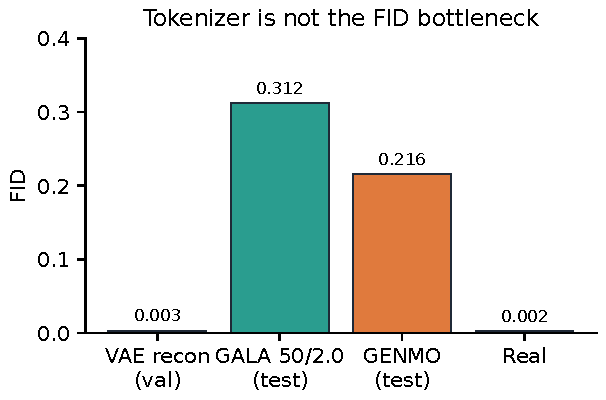
\includegraphics[width=\columnwidth]{fig_recon_gap.pdf}
\caption{Val VAE reconstruction FID versus generated test FID. The tokenizer floor is three orders of magnitude below the generator.}
\label{fig:recon}
\end{figure}

\subsection{Sampling: steps matter more than CFG}

A $3{\times}4$ scan on the full val split (Fig.~\ref{fig:sweep}, Table~\ref{tab:sweep}) was run with the same frozen \texttt{best.pt}.
CFG $=1.0$ collapses both FID and R@3 at every step count: the model was trained with dropout $0.1$ and expects a guided field.
Raising CFG from $2.0$ to $2.5$ at 20 steps \emph{improves} FID slightly ($0.356\to 0.335$) while lifting R@3 to $0.781$; the usual MDM trade (more CFG, worse FID) does not appear until 50 steps.
The FID minimum is \textbf{50 steps, CFG $2.0$} (val FID $0.290$, R@3 $0.753$).
That setting transfers to test as FID $0.312$, R@3 $0.749$---same ranking, a $0.02$ FID val--test gap.

\begin{figure*}[t]
\centering
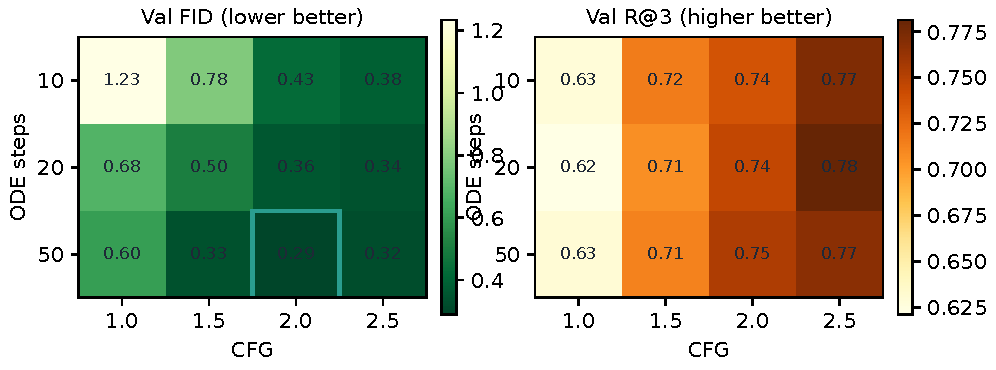
\includegraphics[width=\textwidth]{fig_sweep.pdf}
\caption{Val scan (1504 clips, 1 replication). Teal box: FID-best cell, used for the official 20-rep test.}
\label{fig:sweep}
\end{figure*}

\begin{table}[t]
\centering
\caption{Val sampling scan, 1504 clips, one seed. Official test uses the starred row.}
\label{tab:sweep}
\small
\setlength{\tabcolsep}{3.4pt}
\begin{tabular}{@{}ccccc@{}}
\toprule
Steps & CFG & FID $\downarrow$ & R@3 $\uparrow$ & MM Dist $\downarrow$ \\
\midrule
10 & $1.0$ & $1.233$ & $0.628$ & $4.062$ \\
10 & $2.5$ & $0.382$ & $0.771$ & $3.204$ \\
20 & $2.5$ & $0.335$ & $0.781$ & $3.164$ \\
50 & $1.5$ & $0.331$ & $0.712$ & $3.500$ \\
\textbf{50} & $\mathbf{2.0}$ & $\mathbf{0.290}$ & $0.753$ & $3.301$ \\
50 & $2.5$ & $0.322$ & $0.767$ & $3.177$ \\
\bottomrule
\end{tabular}
\end{table}

\subsection{Training dynamics}

Fig.~\ref{fig:train} is the 320-clip, 10-step val used to pick \texttt{best.pt}.
FID bottoms at step 35k ($0.41$) and never returns; R@3 continues to $0.784$ at 90k.
The checkpoint we evaluate is therefore FID-optimal under a cheaper protocol than the one in Table~\ref{tab:main}.
A matched 20-step val plus EMA is wired for the next run and is not claimed here.

\begin{figure}[t]
\centering
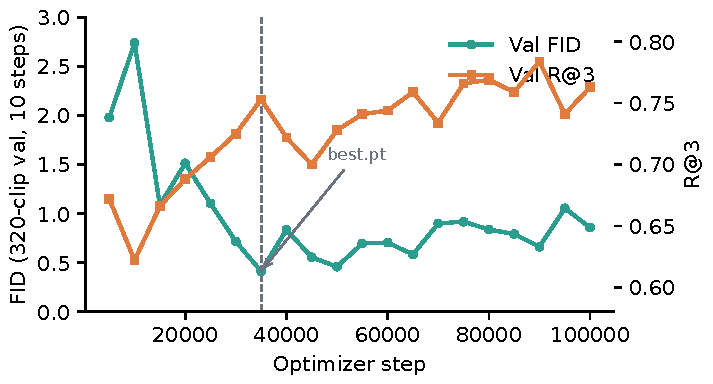
\includegraphics[width=\columnwidth]{fig_train_curve.pdf}
\caption{Online val during Flow training (320 clips, 10 Euler steps, CFG $2.5$). \texttt{best.pt} is the FID minimum at 35k steps.}
\label{fig:train}
\end{figure}

\section{Limitations}

FID $0.31$ is not competitive with EMDM~\cite{zhou2024emdm}, T2M-GPT~\cite{zhang2023t2mgpt}, or MoMask~\cite{guo2024momask}.
The DiT is 8 layers; effective batch 16; no EMA in the evaluated weights; val selection used 10 steps on 320 clips.
CFG and step count were tuned on val then frozen; that is still a form of test-set leakage at the hyperparameter level.
KIT-ML official Guo numbers are not in this draft.
We did not re-run GENMO; we compare to their published Table~4.

\section{Conclusion}

GALA is a graph-aware latent flow that, on the official HumanML3D test, beats GENMO and MDM on text alignment and matches real Diversity, while remaining behind GENMO and EMDM on FID.
The tokenizer is essentially lossless; the remaining error is in the flow ODE.
Fifty Euler steps at CFG $2.0$ is the best FID we can extract from the current weights without retraining.
The next weights should be selected under the same 20-step protocol used at test time, with EMA.

\bibliographystyle{unsrtnat}
\bibliography{references}

\end{document}
